\documentclass[a4paper,11pt]{article}
\usepackage{tikz-cd}
\usepackage{tikz}

\begin{document}

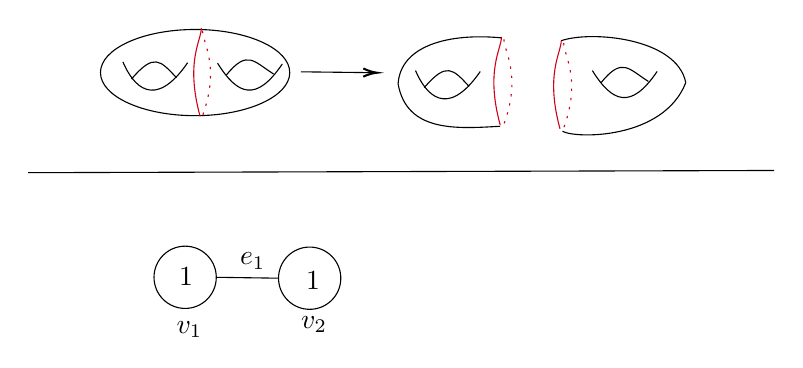
\begin{tikzpicture}[x=0.45pt,y=0.45pt,yscale=-1,xscale=1]

\draw   (100,141.61) .. controls (100,122.5) and (134.03,107) .. (176,107) .. controls (217.97,107) and (252,122.5) .. (252,141.61) .. controls (252,160.72) and (217.97,176.22) .. (176,176.22) .. controls (134.03,176.22) and (100,160.72) .. (100,141.61) -- cycle ;
\draw    (201,143.72) .. controls (218,122.72) and (223,132.72) .. (239,142.72) ;
\draw    (125,146.72) .. controls (143,125.72) and (148,131.72) .. (161,145.72) ;
\draw    (194,134) .. controls (210,159.72) and (225,165.72) .. (246,134.72) ;
\draw    (118,133) .. controls (126,151.72) and (143,172.72) .. (170,133.72) ;
\draw [color={rgb, 255:red, 208; green, 2; blue, 27 }  ,draw opacity=1 ]   (181,106) .. controls (181,115.72) and (168,132.72) .. (180,176.72) ;
\draw [color={rgb, 255:red, 208; green, 2; blue, 27 }  ,draw opacity=1 ] [dash pattern={on 0.84pt off 2.51pt}]  (182,108) .. controls (182,117.72) and (197,137.72) .. (181,178.72) ;
\draw    (261,141) -- (320,141.7) ;
\draw [shift={(322,141.72)}, rotate = 180.68] [color={rgb, 255:red, 0; green, 0; blue, 0 }  ][line width=0.75]    (10.93,-3.29) .. controls (6.95,-1.4) and (3.31,-0.3) .. (0,0) .. controls (3.31,0.3) and (6.95,1.4) .. (10.93,3.29)   ;
\draw [color={rgb, 255:red, 208; green, 2; blue, 27 }  ,draw opacity=1 ]   (422,113) .. controls (422,122.72) and (409,139.72) .. (421,183.72) ;
\draw [color={rgb, 255:red, 208; green, 2; blue, 27 }  ,draw opacity=1 ] [dash pattern={on 0.84pt off 2.51pt}]  (424,115) .. controls (424,124.72) and (439,144.72) .. (423,185.72) ;
\draw    (339,150.72) .. controls (341,119.72) and (380,109.72) .. (422,113.72) ;
\draw    (339,150.72) .. controls (346,189.72) and (386,186.72) .. (421,184.72) ;
\draw    (360,153.72) .. controls (378,132.72) and (383,138.72) .. (396,152.72) ;
\draw    (353,140) .. controls (361,158.72) and (378,179.72) .. (405,140.72) ;
\draw    (471,188.72) .. controls (481,194.72) and (552,195.72) .. (570,149.72) ;
\draw [color={rgb, 255:red, 208; green, 2; blue, 27 }  ,draw opacity=1 ]   (470,116) .. controls (470,125.72) and (457,142.72) .. (469,186.72) ;
\draw [color={rgb, 255:red, 208; green, 2; blue, 27 }  ,draw opacity=1 ] [dash pattern={on 0.84pt off 2.51pt}]  (472,118) .. controls (472,127.72) and (487,147.72) .. (471,188.72) ;

\draw    (470,116) .. controls (494,107.72) and (563,113.72) .. (570,149.72) ;
\draw    (502,149.72) .. controls (519,128.72) and (524,138.72) .. (540,148.72) ;
\draw    (495,140) .. controls (511,165.72) and (526,171.72) .. (547,140.72) ;
\draw   (143,306) .. controls (143,292.19) and (154.19,281) .. (168,281) .. controls (181.81,281) and (193,292.19) .. (193,306) .. controls (193,319.81) and (181.81,331) .. (168,331) .. controls (154.19,331) and (143,319.81) .. (143,306) -- cycle ;
\draw    (193,306) -- (243,306.72) ;
\draw   (243,306.72) .. controls (243,292.91) and (254.19,281.72) .. (268,281.72) .. controls (281.81,281.72) and (293,292.91) .. (293,306.72) .. controls (293,320.53) and (281.81,331.72) .. (268,331.72) .. controls (254.19,331.72) and (243,320.53) .. (243,306.72) -- cycle ;
\draw    (42,222) -- (641,220.22) ;


\draw (161,296.4) node [anchor=north west][inner sep=0.75pt]    {$1$};
% Text Node
\draw (263,299.4) node [anchor=north west][inner sep=0.75pt]    {$1$};
% Text Node
\draw (210,284.4) node [anchor=north west][inner sep=0.75pt]    {$e_{1}$};
% Text Node
\draw (159,339.4) node [anchor=north west][inner sep=0.75pt]    {$v_{1}$};
% Text Node
\draw (259,335.4) node [anchor=north west][inner sep=0.75pt]    {$v_{2}$};


\end{tikzpicture}

\end{document}